\documentclass[12pt,a4paper]{article}
\usepackage[margin=0.8in]{geometry}
\usepackage{amsmath,amssymb}
\usepackage{array}
\usepackage{booktabs}
\usepackage{fancyhdr}
\usepackage{tikz}
\usetikzlibrary{positioning,shapes,arrows}

\pagestyle{fancy}
\fancyhf{}
\renewcommand{\headrulewidth}{0pt}

\begin{document}

\begin{center}
\begin{tabular}{|c|c|c|c|c|c|c|c|c|c|}
\hline
\multicolumn{10}{|c|}{USN} \\
\hline
& & & & & & & & & \\
\hline
\end{tabular}

\vspace{0.4cm}

{\Large \textbf{NMAM INSTITUTE OF TECHNOLOGY, NITTE}}\\[0.2cm]
{\small \textit{(An Autonomous Institution affiliated to VTU, Belagavi)}}\\[0.2cm]
{\large \textbf{IV Sem B.E. (CSE/ISE/AIM/CCE) Mid Semester Examinations - II, July 2023}}\\[0.2cm]
{\large \textbf{20CS402 / 21IS402 / 21AM402 / 21CC402 -- DESIGN AND ANALYSIS OF ALGORITHMS}}\\[0.2cm]
\end{center}

\noindent
\begin{tabular}{p{8cm}r}
\textbf{Duration:} 1 Hour & \textbf{Max. Marks:} 20
\end{tabular}

\vspace{0.2cm}
\begin{center}
\textit{Note: Answer any \textbf{One} full question from \textbf{each Unit}.}
\end{center}

\vspace{0.2cm}

\begin{center}
{\large \textbf{Unit -- I}}
\end{center}

\noindent
\begin{tabular}{|p{10.5cm}|c|c|c|c|}
\hline
\textbf{Question} & \textbf{Marks} & \textbf{BT*} & \textbf{CO*} & \textbf{PO*} \\
\hline
\textbf{1. a)} Traverse the graph below using DFS and BFS. Also write the DFS and BFS tree for the same.

\begin{center}
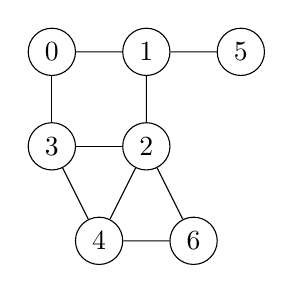
\begin{tikzpicture}[scale=0.8, every node/.style={circle, draw, fill=white, minimum size=6mm, inner sep=1pt}]
\node (0) at (0,2) {0};
\node (1) at (1.5,2) {1};
\node (5) at (3,2) {5};
\node (3) at (0,0.5) {3};
\node (2) at (1.5,0.5) {2};
\node (4) at (0.75,-1) {4};
\node (6) at (2.25,-1) {6};

\draw (0) -- (1);
\draw (0) -- (3);
\draw (1) -- (2);
\draw (1) -- (5);
\draw (3) -- (2);
\draw (3) -- (4);
\draw (2) -- (4);
\draw (2) -- (6);
\draw (4) -- (6);
\end{tikzpicture}
\end{center} & 5 & L*2 & 3 & 1,2 \\
\hline
\textbf{b)} Write insertion sort algorithm and trace it for the following input: \newline ALGORITHMS & 5 & L2 & 3 & 1,2 \\
\hline
\textbf{2. a)} Write the algorithm for BottomUp Heap construction. Apply Heapsort for the following input. Show detailed construction of heap for every step. \textit{Input:} 28 15 45 6 17 32 3 12 & 5 & L2 & 3 & 1,2 \\
\hline
\textbf{b)} Explain the two methods for finding the topological order for any graph. Apply any of the methods to write the topological sort order for following graph.

\begin{center}
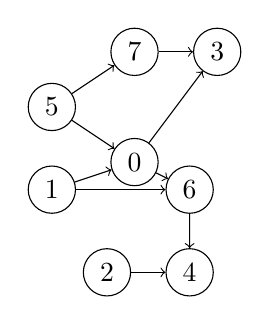
\begin{tikzpicture}[scale=0.7, every node/.style={circle, draw, fill=white, minimum size=6mm, inner sep=1pt}]
\node (5) at (0,1.5) {5};
\node (7) at (1.5,2.5) {7};
\node (3) at (3,2.5) {3};
\node (0) at (1.5,0.5) {0};
\node (1) at (0,0) {1};
\node (6) at (2.5,0) {6};
\node (2) at (1,-1.5) {2};
\node (4) at (2.5,-1.5) {4};

\draw[->] (5) -- (7);
\draw[->] (5) -- (0);
\draw[->] (7) -- (3);
\draw[->] (0) -- (3);
\draw[->] (1) -- (0);
\draw[->] (1) -- (6);
\draw[->] (0) -- (6);
\draw[->] (2) -- (4);
\draw[->] (6) -- (4);
\end{tikzpicture}
\end{center} & 5 & L2 & 3 & 2,3 \\
\hline
\end{tabular}

\vspace{0.3cm}

\begin{center}
{\large \textbf{Unit -- II}}
\end{center}

\noindent
\begin{tabular}{|p{10.5cm}|c|c|c|c|}
\hline
\textbf{Question} & \textbf{Marks} & \textbf{BT*} & \textbf{CO*} & \textbf{PO*} \\
\hline
\textbf{3. a)} Construct AVL Tree for the input given below. Explain the types of rotations used in the construction. \newline 12, 56, 89, 16, 25, 100, 75, 55, 95, 50 & 5 & L2 & 3 & 2,3 \\
\hline
\textbf{b)} Write Horspool's String Matching Algorithm and apply the same for the following input: \textit{Text}: NITTE UNIVERSITY \quad \textit{Pattern}: SIT & 5 & L2 & 4 & 2,3 \\
\hline
\textbf{4. a)} Write Floyds Algorithm and apply the same for the distance matrix given below: (Note: inf stands for infinity) \newline
\begin{tabular}{cccc}
0 & 2 & 4 & 3 \\
5 & 0 & inf & 3 \\
5 & inf & 0 & 3 \\
inf & 1 & 4 & 0
\end{tabular} & 5 & L2 & 4 & 2,3 \\
\hline
\textbf{b)} Construct 2-3 Tree for the input given below. \newline INFORMATIVE & 5 & L2 & 3 & 1,2 \\
\hline
\end{tabular}

\vspace{0.3cm}
\begin{center}
\small{Bloom's Taxonomy, L* Level; CO* Course Outcome; PO* Program Outcome}\\[0.2cm]
******************
\end{center}

\end{document}
